
\documentclass{article}

\usepackage[final]{nips_2017}


\usepackage[utf8]{inputenc} % allow utf-8 input
\usepackage[T1]{fontenc}    % use 8-bit T1 fonts
\usepackage{graphicx}
\usepackage{algpseudocode}
\usepackage{algorithm}
\graphicspath{ {images/} }
\usepackage{hyperref}       % hyperlinks
\usepackage{url}            % simple URL typesetting
\usepackage{booktabs}       % professional-quality tables
\usepackage{amsfonts}       % blackboard math symbols
\usepackage{nicefrac}       % compact symbols for 1/2, etc.
\usepackage{microtype}      % microtypography

\title{Simulating Game Agent using Q-Network
(Reinforcement Learning Technique)}

\author{
  Advait Trivedi \\
  \texttt{astrived} \\
  \AND
  Sainag Shetty \\
  \texttt{sgshetty} \\
   \And
  Aaroh Gala \\
  \texttt{agala} \\
  \And
  Pratik Kumar Jain \\
  \texttt{pjain22} \\
}

\begin{document}
% \nipsfinalcopy is no longer used

\maketitle
\section{Introduction}

In this digital age, data grows at an exponential rate.  Data Mining techniques have now become  a mainstream tool to comprehend and visualize information. Traditional machine learning strategies often rely on mathematical and statistical methods to define result. However, a human supervision and domain expertise is a major dependency for such solutions. Data pre-processing and feature engineering often come at a great cost to structure the exabytes of unstructured raw data every business use case deals with. Thus, to keep up with such fast paced scaling of data we must adopt smarter strategies to tackle unstructured data dumps. Reinforcement learning is one such way to do so.

Philosophically, most forms of intelligence learn through different life experiences which comes at a cost. Reinforcement learning follows a similar strategy where a policy creation is guided by a cost metric assessing it’s actions. It is popularly used to train Game AI. Similar policies can be extrapolated to find optimal results in the field of econometrics and supply chain managements. An interesting Reinforcement learning technique for building Game AI is Q-Learning which is the main focus of our project.

Q-learning is a type of reinforcement learning technique that minimizes behaviour of a learning agent through a cost estimated error table. Since most real world problems or at times even game state problems can grow very large, our table based model would struggle to scale. To overcome this we used a neural network as a function approximator, mapping input states to output Q-action values.

The proposed project endeavors to train a Deep Q-network which takes its inspiration from the Deep Minds Atari Game playing paper[1] to simulate a game agent to play the popular game flappy bird. Our experimental setup has been run for several epochs to enable the agent to adopt a better game playing strategy.


\section{Background}

Q-learning is a model-free reinforcement learning technique. The use of Q- learning is to find an optimal action-selection policy for any given Markov decision process (MDP). It learns using an action-value function that gives the expected benefit of a certain action in a given state and then using the optimality policy. Policy is a rule that is followed by an agent to take an action in a particular state in which the agent is. After learning such an action-value function, construction of the optimal policy is done by selecting the action which has the highest value in all the state.

Equation of Q-learning is represented in Figure 1 . The core of the policy is a simple value iteration update using a weighted average of the old value and the new information. The Q update is made in the direction of the current reward and a discounted estimation of maximal future reward for a certain series of action state transition. Here α is the learning rate often assuming values between (0,1]. Gamma is the discount factor. Q-learning control always converges to the optimal action-value function.

\begin{figure}[H]
  \centering
      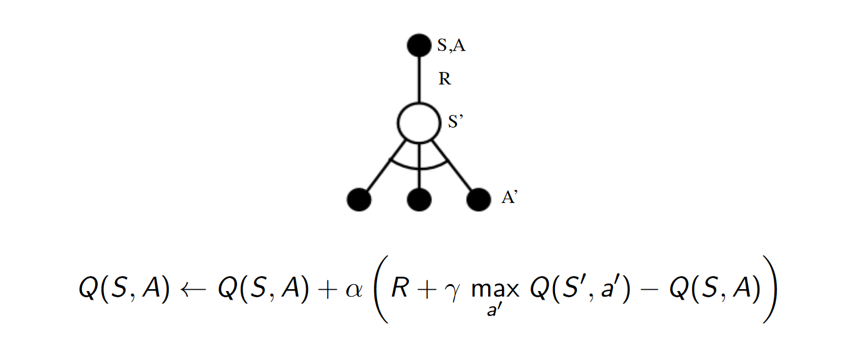
\includegraphics{f1}
  \caption{Figurative representation of Q-Learning Control Update}
\end{figure}

Among all, the important thing of Q-learning is that it is able to compare the expected output of the available actions without requiring a model of the environment. Also, Q-learning can handle problems with stochastic transitions and rewards, without any need to change it. It has been proven that Q-learning eventually finds an optimal policy[2], in the sense that the expected value of the total reward return over all successive steps, starting from the current state, is the maximum achievable for any finite MDP.

In the paper, Playing Atari with Deep Reinforcement Learning, DeepMind demonstrated how a Computer learned to play an Atari 2600 games by just observing the environments screen pixels and receiving rewards when the score in the game increased. The obtained results by this was remarkable because the games and goals in each were different and to obtained such results were very difficult for humans. After achieving these outputs they used the same model architecture to learn seven different games and the among these seven the algorithm works better than humans in three of them.[1]


\section{Method}

Our game simulation involves dynamic state changes depending on the position of the bird in that frame. Since the frame after downsizing are represented as a 80X80 pixel grid, and 4 such stacked frames are taken as image inputs, our traditional Q-Learner would have a Q table whose size would be computationally unfeasible to work with. Taking the suggestion of Silver et al.[2], a neural network could be used to represent structured features covering the state-action space instead.

Deep neural networks have exhibited dexterity over computer vision and speech recognition problems when trained on substantially large training sets. Convoluted networks have facilitated a paradigm shift of using directly raw input images instead of handcrafted image feature inputs while dealing with image segmentation and classification problem[6]. These successes motivate the use of direct image input strategy for training our reinforcement learning agent.

 Our goal is to connect a reinforcement learning algorithm to a deep neural network which operates directly on RGB images and efficiently process training data by using adam updates. The architecture utilize a technique known as experience replay [7] where the agent’s experiences  is memorized to be pooled over many episodes into a replay memory. Q-learning updates as minibatch updates are applied to samples of experience, drawn at random from the pool of stored samples. After performing experience replay, the agent selects and executes an action according to an ε-greedy policy. Since using histories of arbitrary length as inputs to a neural network can be difficult, our Q-function instead works on fixed length representation of histories produced by a function ϕ. 
 
This approach has several advantages over standard online Q-learning [3]. First, each step of experience is potentially used in many weight updates, which allows for greater data efficiency. By using experience replay the behavior distribution is averaged over many of its previous states, smoothing out learning and avoiding oscillations or divergence in the parameters. Note that when learning by experience replay, it is necessary to learn off-policy (because our current parameters are different to those used to generate the sample), which motivates the choice of Q-learning.


We have used the following algorithm for implementation of the project.

\begin{algorithm}[H]
  \caption{Deep Q-learning with Experience Replay }

  \begin{algorithmic}
    \State Initialize replay memory D to capacity N
    \State Initialize action-value function Q with random weights 
    \For  {episode = 1, M} 
    \State Initialise sequence s1 = x1 and preprocessed sequenced  $\phi$1 = $\phi$(s1)
    \For  {t = 1, T } 
    \State With probability $\epsilon$ select a random action at
\State otherwise select at = maxa Q$\times$($\phi$(st), a; $\theta$)
\State Execute action at in emulator and observe reward rt and image xt+1 
\State Set st+1 = st, at, xt+1 and preprocess $\phi$t+1 = $\phi$(st+1)
\State Store transition ($\phi$t, at, rt, $\phi$+1) in D
\State Sample random minibatch of transitions ($\phi$j , aj , rj , $\phi$j +1 ) from D 
\State \begin{center}
    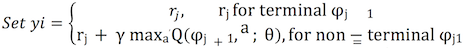
\includegraphics{algo1}
\end{center}
\State Perform gradient descent step on (yj  - Q($\phi$j , aj ; $\theta$))2 according to equation 3

\EndFor
    \EndFor
  \end{algorithmic}
\end{algorithm}

\section{Experiment}

In this project, we demonstrate the use of Deep Q-Learning algorithm and Keras to run the game of Flappy Bird. 

\subsection{Agent Data Gathering and Environment Simulation}

The 2013 mobile application game “Flappy Bird” has been simulated in python using pygames. The game involves a bird trying to pass through tunnels to maximize the score in the game. The bird has a constant horizontal velocity. The action space involved to control the bird are flap or no flap. A flap results in a constant vertical rise of the bird from its current position. A no flap followed by a subsequent flap action will result in no vertical position change. A no flap followed by a no flap results in the vertical fall from its current position.

Action Space for the agent = {Flap: Represented by 1, No Flap:Respresented by 0}
The reward scheme designed for learning purposes is :
\begin{center}
    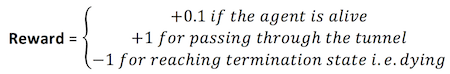
\includegraphics{expt1}
\end{center}

\textbf{Agent Data Gathering}: The Q-learner interacts with the Game API to receive inputs: Image frame, reward for current state and Boolean value of termination. The tunnels are generated at random by the simulator. The deep Q-network architecture learns positional data of the game state due to enhanced feature generation handled by the convolutional layers. To make computations lighter, we preprocess the image by scaling it down to a 80X80 grayscale representation. Since the agent needs a sense of velocity of the bird moving ahead, the experiment stacks 4 such image frames into one for learning purposes. The agent constantly updates the replay memory as the simulator returns the outcome of the action selected for a given state.

\begin{figure}[H]
  \centering
      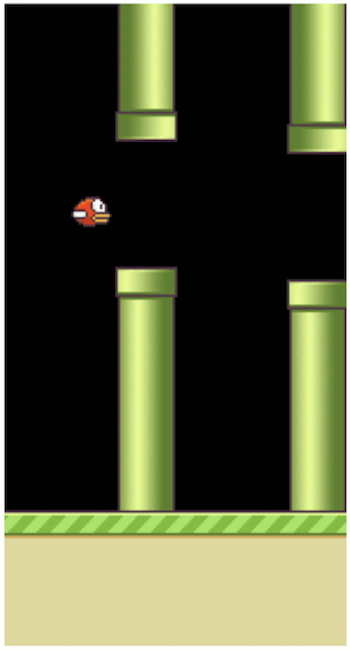
\includegraphics{method6}
  \caption{The Enivironment of a Flappy Bird Game}
\end{figure}

\subsection{Neural Network Architecture}

\begin{figure}[H]
  \centering
      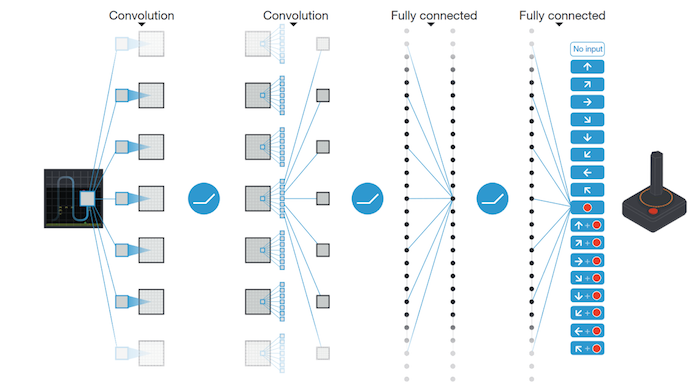
\includegraphics{expt2}
  \caption{Architecture of the neural network is inspired by [2]}
\end{figure}

The input of the network is an image frame of dimension 4X80X80.Here we pass 4 image frames of size 80X80 for learning. The initial convolution layers handle image feature extraction. The subsequent convolution layers give a more human like input representation of the game environment.

\begin{center}
 \begin{tabular}{||c c c||} 
 \hline
 Layer number & Property of layer & Activation Function \\ [0.5ex] 
 \hline\hline
 1st convoluted layer & 32 filters of 8 x 8 with stride 4 & Relu \\ 
 \hline
 2nd Convoluted layer & 64 filters of 4 x 4 with stride 2 & Relu \\
 \hline
 3rd Convoluted layer & 64 filters of 3 x 3 with stride 1 & Relu \\
 \hline
 Fully connected hidden layer & 512 rectifier units & Relu \\
 \hline
 Output layer & Output unit: Flap/No Flap decision & - \\ [1ex] 
 \hline
\end{tabular}
\end{center}

\subsection{Optimization algorithm}
Adaptive Moment Estimation (Adam) is employed as the optimization algorithm. Adam seemed like a right choice over traditional gradient based optimizers as it computes adaptive learning rates for each parameter whilst maintaining a record of  an exponentially decaying average of past gradients and squared gradients. This is the reason it outperforms  other adaptive technique[5]. The learning rate is 1.e-6. We have considered mean squared error as the loss function.

\subsection{Experience replay and Decay Rate}
To improve stability of the Deep Q Network, a replay data structure is used, hoarding all state, action, reward, next state transitions. The learner will randomly select a minibatch of size = 32 to get better results. 

The Q-learner is fed with a positive decay rate of 0.99 ($\gamma$ = 0.99). Since for this case, our current state choice could suddenly lead to termination, the idea is to make hoices that definitely do not result in our bird's death.

\subsection{Exploration vs Exploitation (epsilon-greedy policy)}
In Reinforcement learning, a popular dilemma for the agent is to explore new action spaces or rely on previous learner. We can tackle this by choosing a greedy approach. A popular approach is called $\epsilon$ greedy approach, in which the policy incorporates exploring a  random action some percentage of the time, as dictated by $\epsilon$ (0,1). The strategy will help the RL agent to occasionally try something new and see if we can achieve ultimate strategy. We have adopted to dynamically reduce the epsilon value from an initial value of 0.9 on every epoch. The objective is, with more epochs, we want our agent to rely more on its experience. 


\section{Results}
After developing the game environment, we trained the agent to learn the environment and perform actions accordingly. Due to unavailability of GPU and time constraints, we ran the experiment on the following software and hardware configurations:
Hardware : Processor - 3.1 GHz Intel Core i5 Dual Core
Software : macOS High Sierra version 10.13.1.
We trained the agent for 15 epochs where each epoch corresponds to 10000 timestamps. Each epoch took around an hour of training time. Out of this, 15 epochs, the first half of epoch 1 was the observe time where the agent observed the environment in which it was running. Later the agent started exploring the environment by performing different actions such as flap or no flap. We calculated the Qmax value for every timestamp, and stored the average for each epoch. The following Figure 3 shows a plot of Average Qmax value with number of epochs. From the figure, we can see that the value of average Qmax increases as the number of epochs increases.

\begin{figure}[H]
  \centering
      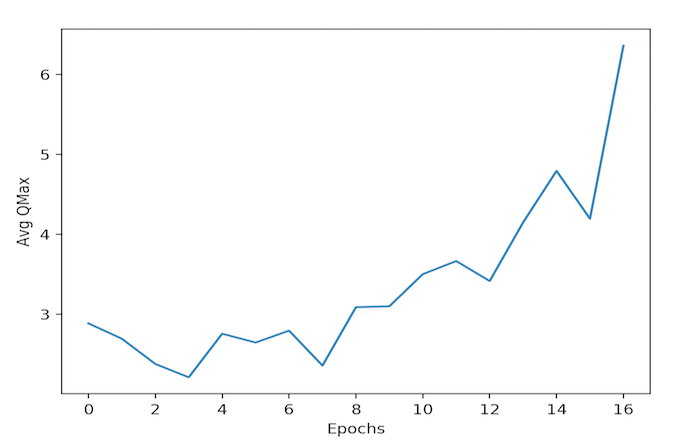
\includegraphics{res2}
  \caption{A plot showing the increase in the value of Average Qmax as Epochs increases where every epochs corresponds to 10000 timestampms.}
\end{figure}

Along with the increase in the Qmax value, the agent also learned to stay alive for a longer period of time by optimisng the weights and taking actions according to that. This can be seen from Figure 4 which shows a snapshot of the agent successfully passing through the tunnels to stay alive which shows that after 15 epochs the agent has learned to stay alive for a longer period of time. 

\begin{figure}[H]
  \centering
      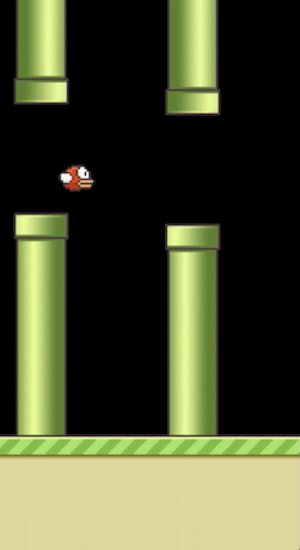
\includegraphics{res3}
  \caption{A snapshot of the agent after learning to play the game successfully}
\end{figure}


\section{Conclusion}

After training the agent for 15 epochs, the agent successfully updates its action policy to achieve a maximum score according to Q-policy updates. Initially a naïve policy of just choosing one action was adopted which produced unfavorable results. As more training iterations go by, the agent started using different combination of actions to increase the Qmax value and because of that it started learning as to which action will help it staying alive. After 15 epochs the agent successfully learned to alternate between flap and no-flap at the right time in the game and stays alive for as long as possible by increasing the reward. An in-game score of 6 can be easily achieved by our current model. 

\section*{References}

\small

[1] \label{pap1}Mnih, V., Kavukcuoglu, K., Silver, D., Graves, A., Antonoglou, I., Wierstra, D. and Riedmiller, M., 2013. Playing atari with deep reinforcement learning. arXiv preprint arXiv:1312.5602.

[2] Mnih, V., Kavukcuoglu, K., Silver, D., Rusu, A.A., Veness, J., Bellemare, M.G., Graves, A., Riedmiller, M., Fidjeland, A.K., Ostrovski, G. and Petersen, S., 2015. Human-level control through deep reinforcement learning. Nature, 518(7540), pp.529-533.

[3] Sutton, R.S. and Barto, A.G., 1998. Reinforcement learning: An introduction (Vol. 1, No. 1). Cambridge: MIT press.

[4] Ponce, H., \& Padilla, R. (2014, November). A hierarchical reinforcement learning based artificial intelli- gence for non-player characters in video games. In Mexican International Conference on Artificial Intelligence (pp. 172-183). Springer, Cham.

[5] Kingma, Diederik, and Jimmy Ba. "Adam: A method for stochastic optimization." arXiv preprint arXiv:1412.6980 (2014).

[6]	Krizhevsky, Alex, Ilya Sutskever, and Geoffrey E. Hinton. "Imagenet classification with deep convolutional neural networks." Advances in neural information processing systems. 2012.

[7]	Lin, Long-Ji. Reinforcement learning for robots using neural networks. No. CMU-CS-93-103. Carnegie-Mellon Univ Pittsburgh PA School of Computer Science, 1993.

<<<<<<< HEAD
\textbf{GitHub Project Link: https://github.ncsu.edu/sgshetty/FlappyBird-QLearn}
=======
\textbf{GitHub Link: https://github.ncsu.edu/sgshetty/FlappyBird-QLearn}
>>>>>>> b43ccae24698bca30e02c70213ff6504d812ae52
\end{document}
